\chapter{Progress of Cavalcanti the Younger}

Meanwhile M. Cavalcanti the elder had returned to his service, not in
the army of his majesty the Emperor of Austria, but at the gaming-table
of the baths of Lucca, of which he was one of the most assiduous
courtiers. He had spent every farthing that had been allowed for his
journey as a reward for the majestic and solemn manner in which he had
maintained his assumed character of father.

M. Andrea at his departure inherited all the papers which proved that
he had indeed the honor of being the son of the Marquis Bartolomeo and
the Marchioness Oliva Corsinari. He was now fairly launched in that
Parisian society which gives such ready access to foreigners, and
treats them, not as they really are, but as they wish to be considered.
Besides, what is required of a young man in Paris? To speak its
language tolerably, to make a good appearance, to be a good gamester,
and to pay in cash. They are certainly less particular with a foreigner
than with a Frenchman. Andrea had, then, in a fortnight, attained a
very fair position. He was called count, he was said to possess 50,000
livres per annum; and his father’s immense riches, buried in the
quarries of Saravezza, were a constant theme. A learned man, before
whom the last circumstance was mentioned as a fact, declared he had
seen the quarries in question, which gave great weight to assertions
hitherto somewhat doubtful, but which now assumed the garb of reality.

Such was the state of society in Paris at the period we bring before
our readers, when Monte Cristo went one evening to pay M. Danglars a
visit. M. Danglars was out, but the count was asked to go and see the
baroness, and he accepted the invitation. It was never without a
nervous shudder, since the dinner at Auteuil, and the events which
followed it, that Madame Danglars heard Monte Cristo’s name announced.
If he did not come, the painful sensation became most intense; if, on
the contrary, he appeared, his noble countenance, his brilliant eyes,
his amiability, his polite attention even towards Madame Danglars, soon
dispelled every impression of fear. It appeared impossible to the
baroness that a man of such delightfully pleasing manners should
entertain evil designs against her; besides, the most corrupt minds
only suspect evil when it would answer some interested end—useless
injury is repugnant to every mind.

\begin{figure}[ht]
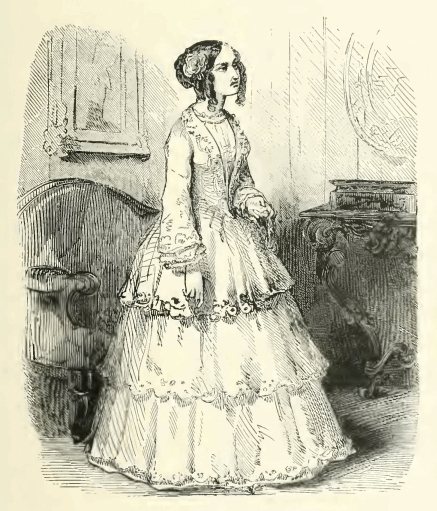
\includegraphics[width=\textwidth]{40048m.jpg}
\end{figure}

When Monte Cristo entered the boudoir, to which we have already once
introduced our readers, and where the baroness was examining some
drawings, which her daughter passed to her after having looked at them
with M. Cavalcanti, his presence soon produced its usual effect, and it
was with smiles that the baroness received the count, although she had
been a little disconcerted at the announcement of his name. The latter
took in the whole scene at a glance.

The baroness was partially reclining on a sofa, Eugénie sat near her,
and Cavalcanti was standing. Cavalcanti, dressed in black, like one of
Goethe’s heroes, with varnished shoes and white silk open-worked
stockings, passed a white and tolerably nice-looking hand through his
light hair, and so displayed a sparkling diamond, that in spite of
Monte Cristo’s advice the vain young man had been unable to resist
putting on his little finger. This movement was accompanied by killing
glances at Mademoiselle Danglars, and by sighs launched in the same
direction.

Mademoiselle Danglars was still the same—cold, beautiful, and
satirical. Not one of these glances, nor one sigh, was lost on her;
they might have been said to fall on the shield of Minerva, which some
philosophers assert protected sometimes the breast of Sappho. Eugénie
bowed coldly to the count, and availed herself of the first moment when
the conversation became earnest to escape to her study, whence very
soon two cheerful and noisy voices being heard in connection with
occasional notes of the piano assured Monte Cristo that Mademoiselle
Danglars preferred to his society and to that of M. Cavalcanti the
company of Mademoiselle Louise d’Armilly, her singing teacher.

It was then, especially while conversing with Madame Danglars, and
apparently absorbed by the charm of the conversation, that the count
noticed M. Andrea Cavalcanti’s solicitude, his manner of listening to
the music at the door he dared not pass, and of manifesting his
admiration.

The banker soon returned. His first look was certainly directed towards
Monte Cristo, but the second was for Andrea. As for his wife, he bowed
to her, as some husbands do to their wives, but in a way that bachelors
will never comprehend, until a very extensive code is published on
conjugal life.

“Have not the ladies invited you to join them at the piano?” said
Danglars to Andrea.

“Alas, no, sir,” replied Andrea with a sigh, still more remarkable than
the former ones. Danglars immediately advanced towards the door and
opened it.

\begin{figure}[ht]
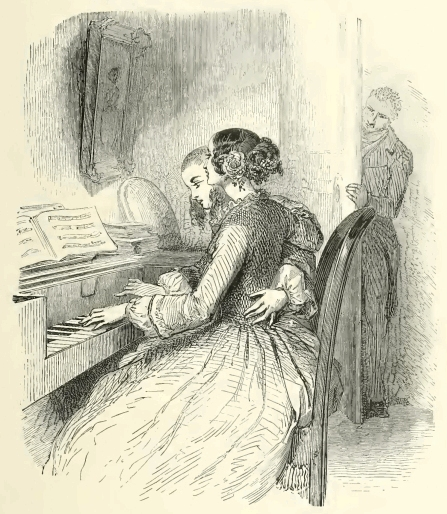
\includegraphics[width=\textwidth]{40050m.jpg}
\end{figure}

The two young ladies were seen seated on the same chair, at the piano,
accompanying themselves, each with one hand, a fancy to which they had
accustomed themselves, and performed admirably. Mademoiselle d’Armilly,
whom they then perceived through the open doorway, formed with Eugénie
one of the \textit{tableaux vivants} of which the Germans are so fond. She was
somewhat beautiful, and exquisitely formed—a little fairy-like figure,
with large curls falling on her neck, which was rather too long, as
Perugino sometimes makes his Virgins, and her eyes dull from fatigue.
She was said to have a weak chest, and like Antonia in the \textit{Cremona
Violin}, she would die one day while singing.

Monte Cristo cast one rapid and curious glance round this sanctum; it
was the first time he had ever seen Mademoiselle d’Armilly, of whom he
had heard much.

“Well,” said the banker to his daughter, “are we then all to be
excluded?”

He then led the young man into the study, and either by chance or
manœuvre the door was partially closed after Andrea, so that from the
place where they sat neither the Count nor the baroness could see
anything; but as the banker had accompanied Andrea, Madame Danglars
appeared to take no notice of it.

The count soon heard Andrea’s voice, singing a Corsican song,
accompanied by the piano. While the count smiled at hearing this song,
which made him lose sight of Andrea in the recollection of Benedetto,
Madame Danglars was boasting to Monte Cristo of her husband’s strength
of mind, who that very morning had lost three or four hundred thousand
francs by a failure at Milan. The praise was well deserved, for had not
the count heard it from the baroness, or by one of those means by which
he knew everything, the baron’s countenance would not have led him to
suspect it.

“Hem,” thought Monte Cristo, “he begins to conceal his losses; a month
since he boasted of them.”

Then aloud,—“Oh, madame, M. Danglars is so skilful, he will soon regain
at the Bourse what he loses elsewhere.”

“I see that you participate in a prevalent error,” said Madame
Danglars.

“What is it?” said Monte Cristo.

“That M. Danglars speculates, whereas he never does.”

“Truly, madame, I recollect M. Debray told me——apropos, what has become
of him? I have seen nothing of him the last three or four days.”

“Nor I,” said Madame Danglars; “but you began a sentence, sir, and did
not finish.”

“Which?”

“M. Debray had told you——”

“Ah, yes; he told me it was you who sacrificed to the demon of
speculation.”

“I was once very fond of it, but I do not indulge now.”

“Then you are wrong, madame. Fortune is precarious; and if I were a
woman and fate had made me a banker’s wife, whatever might be my
confidence in my husband’s good fortune, still in speculation you know
there is great risk. Well, I would secure for myself a fortune
independent of him, even if I acquired it by placing my interests in
hands unknown to him.” Madame Danglars blushed, in spite of all her
efforts.

“Stay,” said Monte Cristo, as though he had not observed her confusion,
“I have heard of a lucky hit that was made yesterday on the Neapolitan
bonds.”

“I have none—nor have I ever possessed any; but really we have talked
long enough of money, count, we are like two stockbrokers; have you
heard how fate is persecuting the poor Villeforts?”

“What has happened?” said the count, simulating total ignorance.

“You know the Marquis of Saint-Méran died a few days after he had set
out on his journey to Paris, and the marchioness a few days after her
arrival?”

“Yes,” said Monte Cristo, “I have heard that; but, as Claudius said to
Hamlet, ‘it is a law of nature; their fathers died before them, and
they mourned their loss; they will die before their children, who will,
in their turn, grieve for them.’”

“But that is not all.”

“Not all!”

“No; they were going to marry their daughter——”

“To M. Franz d’Épinay. Is it broken off?”

“Yesterday morning, it appears, Franz declined the honor.”

“Indeed? And is the reason known?”

“No.”

“How extraordinary! And how does M. de Villefort bear it?”

“As usual. Like a philosopher.”

Danglars returned at this moment alone.

“Well,” said the baroness, “do you leave M. Cavalcanti with your
daughter?”

“And Mademoiselle d’Armilly,” said the banker; “do you consider her no
one?” Then, turning to Monte Cristo, he said, “Prince Cavalcanti is a
charming young man, is he not? But is he really a prince?”

“I will not answer for it,” said Monte Cristo. “His father was
introduced to me as a marquis, so he ought to be a count; but I do not
think he has much claim to that title.”

“Why?” said the banker. “If he is a prince, he is wrong not to maintain
his rank; I do not like anyone to deny his origin.”

“Oh, you are a thorough democrat,” said Monte Cristo, smiling.

“But do you see to what you are exposing yourself?” said the baroness.
“If, perchance, M. de Morcerf came, he would find M. Cavalcanti in that
room, where he, the betrothed of Eugénie, has never been admitted.”

“You may well say, perchance,” replied the banker; “for he comes so
seldom, it would seem only chance that brings him.”

“But should he come and find that young man with your daughter, he
might be displeased.”

“He? You are mistaken. M. Albert would not do us the honor to be
jealous; he does not like Eugénie sufficiently. Besides, I care not for
his displeasure.”

“Still, situated as we are——”

“Yes, do you know how we are situated? At his mother’s ball he danced
once with Eugénie, and M. Cavalcanti three times, and he took no notice
of it.”

The valet announced the Vicomte Albert de Morcerf. The baroness rose
hastily, and was going into the study, when Danglars stopped her.

“Let her alone,” said he.

She looked at him in amazement. Monte Cristo appeared to be unconscious
of what passed. Albert entered, looking very handsome and in high
spirits. He bowed politely to the baroness, familiarly to Danglars, and
affectionately to Monte Cristo. Then turning to the baroness: “May I
ask how Mademoiselle Danglars is?” said he.

“She is quite well,” replied Danglars quickly; “she is at the piano
with M. Cavalcanti.”

Albert retained his calm and indifferent manner; he might feel perhaps
annoyed, but he knew Monte Cristo’s eye was on him. “M. Cavalcanti has
a fine tenor voice,” said he, “and Mademoiselle Eugénie a splendid
soprano, and then she plays the piano like Thalberg. The concert must
be a delightful one.”

“They suit each other remarkably well,” said Danglars. Albert appeared
not to notice this remark, which was, however, so rude that Madame
Danglars blushed.

“I, too,” said the young man, “am a musician—at least, my masters used
to tell me so; but it is strange that my voice never would suit any
other, and a soprano less than any.”

Danglars smiled, and seemed to say, “It is of no consequence.” Then,
hoping doubtless to effect his purpose, he said,—“The prince and my
daughter were universally admired yesterday. You were not of the party,
M. de Morcerf?”

“What prince?” asked Albert.

“Prince Cavalcanti,” said Danglars, who persisted in giving the young
man that title.

“Pardon me,” said Albert, “I was not aware that he was a prince. And
Prince Cavalcanti sang with Mademoiselle Eugénie yesterday? It must
have been charming, indeed. I regret not having heard them. But I was
unable to accept your invitation, having promised to accompany my
mother to a German concert given by the Baroness of Château-Renaud.”

This was followed by rather an awkward silence.

“May I also be allowed,” said Morcerf, “to pay my respects to
Mademoiselle Danglars?”

“Wait a moment,” said the banker, stopping the young man; “do you hear
that delightful cavatina? Ta, ta, ta, ti, ta, ti, ta, ta; it is
charming, let them finish—one moment. Bravo, bravi, brava!” The banker
was enthusiastic in his applause.

\begin{figure}[ht]
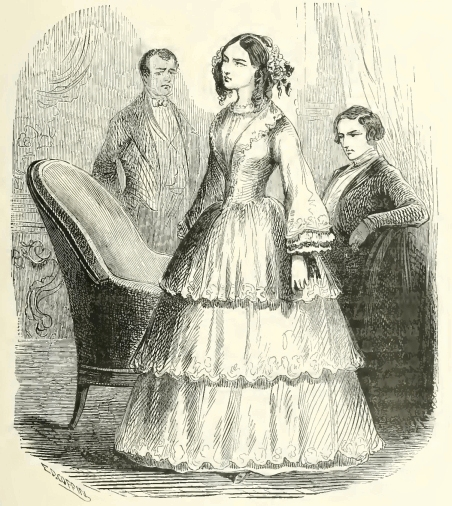
\includegraphics[width=\textwidth]{40054m.jpg}
\end{figure}

“Indeed,” said Albert, “it is exquisite; it is impossible to understand
the music of his country better than Prince Cavalcanti does. You said
prince, did you not? But he can easily become one, if he is not
already; it is no uncommon thing in Italy. But to return to the
charming musicians—you should give us a treat, Danglars, without
telling them there is a stranger. Ask them to sing one more song; it is
so delightful to hear music in the distance, when the musicians are
unrestrained by observation.”

Danglars was quite annoyed by the young man’s indifference. He took
Monte Cristo aside.

“What do you think of our lover?” said he.

“He appears cool. But, then your word is given.”

“Yes, doubtless I have promised to give my daughter to a man who loves
her, but not to one who does not. See him there, cold as marble and
proud like his father. If he were rich, if he had Cavalcanti’s fortune,
that might be pardoned. \textit{Ma foi}, I haven’t consulted my daughter; but
if she has good taste——”

“Oh,” said Monte Cristo, “my fondness may blind me, but I assure you I
consider Morcerf a charming young man who will render your daughter
happy and will sooner or later attain a certain amount of distinction,
and his father’s position is good.”

“Hem,” said Danglars.

“Why do you doubt?”

“The past—that obscurity on the past.”

“But that does not affect the son.”

“Very true.”

“Now, I beg of you, don’t go off your head. It’s a month now that you
have been thinking of this marriage, and you must see that it throws
some responsibility on me, for it was at my house you met this young
Cavalcanti, whom I do not really know at all.”

“But I do.”

“Have you made inquiry?”

“Is there any need of that! Does not his appearance speak for him? And
he is very rich.”

“I am not so sure of that.”

“And yet you said he had money.”

“Fifty thousand livres—a mere trifle.”

“He is well educated.”

“Hem,” said Monte Cristo in his turn.

“He is a musician.”

“So are all Italians.”

“Come, count, you do not do that young man justice.”

“Well, I acknowledge it annoys me, knowing your connection with the
Morcerf family, to see him throw himself in the way.” Danglars burst
out laughing.

“What a Puritan you are!” said he; “that happens every day.”

“But you cannot break it off in this way; the Morcerfs are depending on
this union.”

“Indeed.”

“Positively.”

“Then let them explain themselves; you should give the father a hint,
you are so intimate with the family.”

“I?—where the devil did you find out that?”

“At their ball; it was apparent enough. Why, did not the countess, the
proud Mercédès, the disdainful Catalane, who will scarcely open her
lips to her oldest acquaintances, take your arm, lead you into the
garden, into the private walks, and remain there for half an hour?”

“Ah, baron, baron,” said Albert, “you are not listening—what barbarism
in a megalomaniac like you!”

“Oh, don’t worry about me, Sir Mocker,” said Danglars; then turning to
Monte Cristo he said:

“But will you undertake to speak to the father?”

“Willingly, if you wish it.”

“But let it be done explicitly and positively. If he demands my
daughter let him fix the day—declare his conditions; in short, let us
either understand each other, or quarrel. You understand—no more
delay.”

“Yes, sir, I will give my attention to the subject.”

“I do not say that I await with pleasure his decision, but I do await
it. A banker must, you know, be a slave to his promise.” And Danglars
sighed as M. Cavalcanti had done half an hour before.

“Bravi! bravo! brava!” cried Morcerf, parodying the banker, as the
selection came to an end. Danglars began to look suspiciously at
Morcerf, when someone came and whispered a few words to him.

“I shall soon return,” said the banker to Monte Cristo; “wait for me. I
shall, perhaps, have something to say to you.” And he went out.

The baroness took advantage of her husband’s absence to push open the
door of her daughter’s study, and M. Andrea, who was sitting before the
piano with Mademoiselle Eugénie, started up like a jack-in-the-box.
Albert bowed with a smile to Mademoiselle Danglars, who did not appear
in the least disturbed, and returned his bow with her usual coolness.
Cavalcanti was evidently embarrassed; he bowed to Morcerf, who replied
with the most impertinent look possible. Then Albert launched out in
praise of Mademoiselle Danglars’ voice, and on his regret, after what
he had just heard, that he had been unable to be present the previous
evening.

Cavalcanti, being left alone, turned to Monte Cristo.

“Come,” said Madame Danglars, “leave music and compliments, and let us
go and take tea.”

“Come, Louise,” said Mademoiselle Danglars to her friend.

They passed into the next drawing-room, where tea was prepared. Just as
they were beginning, in the English fashion, to leave the spoons in
their cups, the door again opened and Danglars entered, visibly
agitated. Monte Cristo observed it particularly, and by a look asked
the banker for an explanation.

“I have just received my courier from Greece,” said Danglars.

“Ah, yes,” said the count; “that was the reason of your running away
from us.”

“Yes.”

“How is King Otho getting on?” asked Albert in the most sprightly tone.

Danglars cast another suspicious look towards him without answering,
and Monte Cristo turned away to conceal the expression of pity which
passed over his features, but which was gone in a moment.

“We shall go together, shall we not?” said Albert to the count.

“If you like,” replied the latter.

Albert could not understand the banker’s look, and turning to Monte
Cristo, who understood it perfectly,—“Did you see,” said he, “how he
looked at me?”

“Yes,” said the count; “but did you think there was anything particular
in his look?”

“Indeed, I did; and what does he mean by his news from Greece?”

“How can I tell you?”

“Because I imagine you have correspondents in that country.”

Monte Cristo smiled significantly.

“Stop,” said Albert, “here he comes. I shall compliment Mademoiselle
Danglars on her cameo, while the father talks to you.”

“If you compliment her at all, let it be on her voice, at least,” said
Monte Cristo.

“No, everyone would do that.”

“My dear viscount, you are dreadfully impertinent.”

Albert advanced towards Eugénie, smiling.

Meanwhile, Danglars, stooping to Monte Cristo’s ear, “Your advice was
excellent,” said he; “there is a whole history connected with the names
Fernand and Yanina.”

“Indeed?” said Monte Cristo.

“Yes, I will tell you all; but take away the young man; I cannot endure
his presence.”

“He is going with me. Shall I send the father to you?”

“Immediately.”

“Very well.” The count made a sign to Albert and they bowed to the
ladies, and took their leave, Albert perfectly indifferent to
Mademoiselle Danglars’ contempt, Monte Cristo reiterating his advice to
Madame Danglars on the prudence a banker’s wife should exercise in
providing for the future.

M. Cavalcanti remained master of the field.
